\hypertarget{fastaSeqIO_8c}{
\section{Fasta\-Seq\-IO/fasta\-Seq\-IO.c File Reference}
\label{fastaSeqIO_8c}\index{FastaSeqIO/fastaSeqIO.c@{FastaSeqIO/fastaSeqIO.c}}
}
{\tt \#include \char`\"{}fasta\-Seq\-IO.h\char`\"{}}\par
{\tt \#include $<$stdlib.h$>$}\par
{\tt \#include $<$string.h$>$}\par
{\tt \#include $<$errno.h$>$}\par


Include dependency graph for fasta\-Seq\-IO.c:\begin{figure}[H]
\begin{center}
\leavevmode
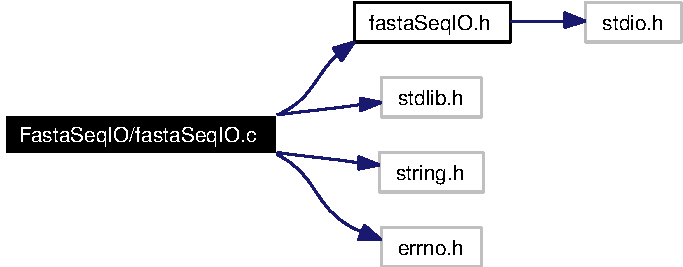
\includegraphics[width=181pt]{fastaSeqIO_8c__incl}
\end{center}
\end{figure}
\subsection*{Data Structures}
\begin{CompactItemize}
\item 
struct \hyperlink{structsSize__t}{s\-Size\_\-t}
\end{CompactItemize}
\subsection*{Defines}
\begin{CompactItemize}
\item 
\#define \hyperlink{fastaSeqIO_8c_a0}{BUFFER}~100000
\item 
\#define \hyperlink{fastaSeqIO_8c_a1}{BIG\_\-BUFFER}~1000000
\end{CompactItemize}
\subsection*{Functions}
\begin{CompactItemize}
\item 
int \hyperlink{fastaSeqIO_8c_a2}{print\-FSeq\-Sub\-Seq} (\hyperlink{structfSeq__t}{f\-Seq\_\-t} $\ast$seq, int start, int stop)
\item 
long \hyperlink{fastaSeqIO_8c_a3}{measure\-Line} (FILE $\ast$INPUT)
\item 
long \hyperlink{fastaSeqIO_8c_a4}{Count\-FSeqs} (FILE $\ast$INPUT)
\item 
long \hyperlink{fastaSeqIO_8c_a5}{count\-Lines} (FILE $\ast$INPUT)
\item 
int \hyperlink{fastaSeqIO_8c_a6}{init\-Aof\-FSeqs} (\hyperlink{structfSeq__t}{f\-Seq\_\-t} $\ast$aos, int num\-Seq)
\item 
char $\ast$$\ast$ \hyperlink{fastaSeqIO_8c_a7}{Read\-File} (FILE $\ast$INPUT, int $\ast$n)
\item 
\hyperlink{structfSeq__t}{f\-Seq\_\-t} $\ast$ \hyperlink{fastaSeqIO_8c_a8}{Read\-Txt\-Seqs} (FILE $\ast$INPUT, int $\ast$number\-Of\-Sequences)
\item 
\hyperlink{structfSeq__t}{f\-Seq\_\-t} $\ast$ \hyperlink{fastaSeqIO_8c_a9}{Read\-FSeqs} (FILE $\ast$INPUT, int $\ast$number\-Of\-Sequences)
\item 
int \hyperlink{fastaSeqIO_8c_a10}{Free\-FSeqs} (\hyperlink{structfSeq__t}{f\-Seq\_\-t} $\ast$array\-Of\-Sequences, int number\-Of\-Sequences)
\item 
int \hyperlink{fastaSeqIO_8c_a11}{Write\-FSeq\-A} (FILE $\ast$MY\_\-FILE, \hyperlink{structfSeq__t}{f\-Seq\_\-t} $\ast$array\-Of\-Sequences, int start, int stop)
\end{CompactItemize}


\subsection*{Define Documentation}
\hypertarget{fastaSeqIO_8c_a1}{
\index{fastaSeqIO.c@{fasta\-Seq\-IO.c}!BIG_BUFFER@{BIG\_\-BUFFER}}
\index{BIG_BUFFER@{BIG\_\-BUFFER}!fastaSeqIO.c@{fasta\-Seq\-IO.c}}
\subsubsection[BIG\_\-BUFFER]{\setlength{\rightskip}{0pt plus 5cm}\#define BIG\_\-BUFFER~1000000}}
\label{fastaSeqIO_8c_a1}




Definition at line 11 of file fasta\-Seq\-IO.c.\hypertarget{fastaSeqIO_8c_a0}{
\index{fastaSeqIO.c@{fasta\-Seq\-IO.c}!BUFFER@{BUFFER}}
\index{BUFFER@{BUFFER}!fastaSeqIO.c@{fasta\-Seq\-IO.c}}
\subsubsection[BUFFER]{\setlength{\rightskip}{0pt plus 5cm}\#define BUFFER~100000}}
\label{fastaSeqIO_8c_a0}




Definition at line 10 of file fasta\-Seq\-IO.c.

\subsection*{Function Documentation}
\hypertarget{fastaSeqIO_8c_a4}{
\index{fastaSeqIO.c@{fasta\-Seq\-IO.c}!CountFSeqs@{CountFSeqs}}
\index{CountFSeqs@{CountFSeqs}!fastaSeqIO.c@{fasta\-Seq\-IO.c}}
\subsubsection[CountFSeqs]{\setlength{\rightskip}{0pt plus 5cm}long Count\-FSeqs (FILE $\ast$ {\em INPUT})}}
\label{fastaSeqIO_8c_a4}




Definition at line 44 of file fasta\-Seq\-IO.c.

\scriptsize\begin{verbatim}45 {
46     long start;
47     long count = 0;
48     int myChar;
49     int newLine = 1;
50     start = ftell(INPUT);
51     myChar = fgetc(INPUT);
52     while (myChar != EOF) {
53         if (newLine == 1 && myChar == '>') {
54             count++;
55         }
56         if (myChar == '\n') {
57             newLine = 1;
58         } else {
59             newLine = 0;
60         }
61         myChar = fgetc(INPUT);
62     }
63     fseek(INPUT, start, SEEK_SET);
64     return count;
65 }
\end{verbatim}
\normalsize 


\hypertarget{fastaSeqIO_8c_a5}{
\index{fastaSeqIO.c@{fasta\-Seq\-IO.c}!countLines@{countLines}}
\index{countLines@{countLines}!fastaSeqIO.c@{fasta\-Seq\-IO.c}}
\subsubsection[countLines]{\setlength{\rightskip}{0pt plus 5cm}long count\-Lines (FILE $\ast$ {\em INPUT})}}
\label{fastaSeqIO_8c_a5}




Definition at line 69 of file fasta\-Seq\-IO.c.

Referenced by Read\-File().

\scriptsize\begin{verbatim}70 {
71     long start;
72     long count = 1;
73     int myChar;
74     int status = 0;
75     start = ftell(INPUT);
76     myChar = fgetc(INPUT);
77     while (myChar != EOF) {
78         if (myChar == '\n') {
79             count++;
80             status = 1;
81         } else {
82             status = 0;
83         }
84         myChar = fgetc(INPUT);
85     }
86     if (status == 1) {
87         count--;
88     }
89     fseek(INPUT, start, SEEK_SET);
90     return count;
91 }
\end{verbatim}
\normalsize 


\hypertarget{fastaSeqIO_8c_a10}{
\index{fastaSeqIO.c@{fasta\-Seq\-IO.c}!FreeFSeqs@{FreeFSeqs}}
\index{FreeFSeqs@{FreeFSeqs}!fastaSeqIO.c@{fasta\-Seq\-IO.c}}
\subsubsection[FreeFSeqs]{\setlength{\rightskip}{0pt plus 5cm}int Free\-FSeqs (\hyperlink{structfSeq__t}{f\-Seq\_\-t} $\ast$ {\em array\-Of\-Sequences}, int {\em number\-Of\-Sequences})}}
\label{fastaSeqIO_8c_a10}




Definition at line 304 of file fasta\-Seq\-IO.c.

References f\-Seq\_\-t::label, and f\-Seq\_\-t::seq.

Referenced by main().

\scriptsize\begin{verbatim}305 {
306     int i;
307     for (i = 0; i < numberOfSequences; i++) {
308         if (arrayOfSequences[i].label != NULL) {
309             free(arrayOfSequences[i].label);
310         }
311         arrayOfSequences[i].label = NULL;
312 
313         if (arrayOfSequences[i].seq != NULL) {
314             free(arrayOfSequences[i].seq);
315         }
316         arrayOfSequences[i].seq = NULL;
317     }
318     if (arrayOfSequences != NULL) {
319         free(arrayOfSequences);
320     }
321     arrayOfSequences = NULL;
322     return EXIT_SUCCESS;
323 }
\end{verbatim}
\normalsize 


\hypertarget{fastaSeqIO_8c_a6}{
\index{fastaSeqIO.c@{fasta\-Seq\-IO.c}!initAofFSeqs@{initAofFSeqs}}
\index{initAofFSeqs@{initAofFSeqs}!fastaSeqIO.c@{fasta\-Seq\-IO.c}}
\subsubsection[initAofFSeqs]{\setlength{\rightskip}{0pt plus 5cm}int init\-Aof\-FSeqs (\hyperlink{structfSeq__t}{f\-Seq\_\-t} $\ast$ {\em aos}, int {\em num\-Seq})}}
\label{fastaSeqIO_8c_a6}




Definition at line 94 of file fasta\-Seq\-IO.c.

References f\-Seq\_\-t::label, and f\-Seq\_\-t::seq.

Referenced by Read\-FSeqs(), and Read\-Txt\-Seqs().

\scriptsize\begin{verbatim}95 {
96     int i;
97     for (i = 0; i < numSeq; i++) {
98         aos[i].seq = NULL;
99         aos[i].label = NULL;
100     }
101     return 1;
102 }
\end{verbatim}
\normalsize 


\hypertarget{fastaSeqIO_8c_a3}{
\index{fastaSeqIO.c@{fasta\-Seq\-IO.c}!measureLine@{measureLine}}
\index{measureLine@{measureLine}!fastaSeqIO.c@{fasta\-Seq\-IO.c}}
\subsubsection[measureLine]{\setlength{\rightskip}{0pt plus 5cm}long measure\-Line (FILE $\ast$ {\em INPUT})}}
\label{fastaSeqIO_8c_a3}




Definition at line 25 of file fasta\-Seq\-IO.c.

Referenced by Read\-File().

\scriptsize\begin{verbatim}26 {
27     long start;
28     long count = 0;
29     int myChar;
30     start = ftell(INPUT);
31     myChar = fgetc(INPUT);
32     count++;
33     while (myChar != '\n' && myChar != EOF) {
34         count++;
35         myChar = fgetc(INPUT);
36     }
37     fseek(INPUT, start, SEEK_SET);
38     return count;
39 }
\end{verbatim}
\normalsize 


\hypertarget{fastaSeqIO_8c_a2}{
\index{fastaSeqIO.c@{fasta\-Seq\-IO.c}!printFSeqSubSeq@{printFSeqSubSeq}}
\index{printFSeqSubSeq@{printFSeqSubSeq}!fastaSeqIO.c@{fasta\-Seq\-IO.c}}
\subsubsection[printFSeqSubSeq]{\setlength{\rightskip}{0pt plus 5cm}int print\-FSeq\-Sub\-Seq (\hyperlink{structfSeq__t}{f\-Seq\_\-t} $\ast$ {\em seq}, int {\em start}, int {\em stop})}}
\label{fastaSeqIO_8c_a2}




Definition at line 14 of file fasta\-Seq\-IO.c.

References f\-Seq\_\-t::seq.

\scriptsize\begin{verbatim}14                                                  {
15     int i;
16     for(i=start; i<stop; i++){
17         putchar(seq->seq[i]);
18     }
19     return 0;
20 }
\end{verbatim}
\normalsize 


\hypertarget{fastaSeqIO_8c_a7}{
\index{fastaSeqIO.c@{fasta\-Seq\-IO.c}!ReadFile@{ReadFile}}
\index{ReadFile@{ReadFile}!fastaSeqIO.c@{fasta\-Seq\-IO.c}}
\subsubsection[ReadFile]{\setlength{\rightskip}{0pt plus 5cm}char$\ast$$\ast$ Read\-File (FILE $\ast$ {\em INPUT}, int $\ast$ {\em n})}}
\label{fastaSeqIO_8c_a7}




Definition at line 105 of file fasta\-Seq\-IO.c.

References count\-Lines(), and measure\-Line().

Referenced by Read\-FSeqs(), read\-Real\-Data(), and Read\-Txt\-Seqs().

\scriptsize\begin{verbatim}106 {
107     char **buf = NULL;
108     long nl;
109     long tls = 0;
110     int i=0;
111 
112     nl = countLines(INPUT);
113     if( nl == 0){
114         fprintf(stderr, "\nNo sequences! Error!\n\n");
115         fflush(stderr);
116         return NULL;
117     }
118     buf = (char **) malloc ( (int)(nl+1) * sizeof(char *));
119     if ( buf == NULL){
120         fprintf(stderr, "\nMemory Error\n%s\n", strerror(errno));
121         fflush(stderr);
122         exit(0);
123     }
124 
125     //  measure the first line
126     tls = measureLine(INPUT) + 1;
127     if(tls != 0){
128         buf[i] = (char *) malloc ( tls * sizeof(char));
129         if ( buf[i] == NULL){
130             fprintf(stderr, "\nMemory Error\n%s\n", strerror(errno));
131             fflush(stderr);
132             exit(0);
133         }
134     }
135     fgets(buf[i], tls, INPUT);
136     do{
137         if(buf[i][ strlen(buf[i])-1 ] == '\n'){
138             buf[i][ strlen(buf[i])-1 ] = '\0';
139         }
140         tls = measureLine(INPUT) + 1;
141         if(tls != 0){
142             i++;
143             buf[i] = (char *) malloc ( tls * sizeof(char) );
144             if ( buf[i] == NULL){
145                 fprintf(stderr, "\nMemory Error\n%s\n", strerror(errno));
146                 fflush(stderr);
147                 exit(0);
148             }
149         }
150     }while( fgets(buf[i], tls, INPUT) != NULL );
151     free(buf[i]);
152     buf = (char **) realloc ( buf, i * sizeof(char *) );
153     if ( buf == NULL){
154         fprintf(stderr, "\nMemory Error\n%s\n", strerror(errno));
155         fflush(stderr);
156         return NULL;
157     }
158     //  I think that 'i' might actually be the # of lines
159     //  plus one here?  somehow line 131 isn't being freed,
160     //  or at least 2 bytes of it.
161     *n = i;
162     return buf;
163 }
\end{verbatim}
\normalsize 


\hypertarget{fastaSeqIO_8c_a9}{
\index{fastaSeqIO.c@{fasta\-Seq\-IO.c}!ReadFSeqs@{ReadFSeqs}}
\index{ReadFSeqs@{ReadFSeqs}!fastaSeqIO.c@{fasta\-Seq\-IO.c}}
\subsubsection[ReadFSeqs]{\setlength{\rightskip}{0pt plus 5cm}\hyperlink{structfSeq__t}{f\-Seq\_\-t}$\ast$ Read\-FSeqs (FILE $\ast$ {\em INPUT}, int $\ast$ {\em number\-Of\-Sequences})}}
\label{fastaSeqIO_8c_a9}




Definition at line 199 of file fasta\-Seq\-IO.c.

References init\-Aof\-FSeqs(), f\-Seq\_\-t::label, Read\-File(), f\-Seq\_\-t::seq, s\-Size\_\-t::size, s\-Size\_\-t::start, and s\-Size\_\-t::stop.

Referenced by main().

\scriptsize\begin{verbatim}199                                                {
200     int i,j,k;
201     int nl, ns=0;
202     char **buf = NULL;
203     fSeq_t *aos;
204     sSize_t *ss;
205     sSize_t *ll;
206 
207     buf = ReadFile(INPUT, &nl);
208     if(buf == NULL){
209         return NULL;
210     }
211 
212     //  Count how many sequences we have
213     for( j=0 ; j<nl ; j++){
214         if(buf[j][0] == '>'){
215             ns++;
216         }
217     }
218     ss = (sSize_t *) malloc ( ns * sizeof(sSize_t) );
219     if(ss == NULL){
220         fprintf(stderr, "\nMemory Error\n%s\n", strerror(errno));
221         fflush(stderr);
222         exit(0);
223     }
224     ll = (sSize_t *) malloc ( ns * sizeof(sSize_t) );
225     if(ll == NULL){
226         fprintf(stderr, "\nMemory Error\n%s\n", strerror(errno));
227         fflush(stderr);
228         exit(0);
229     }
230 
231     //  find the first sequence
232     k=0;
233     while( buf[k][0] != '>'){
234         k++;
235     }
236 
237     //  record how large each sequence is
238     i = -1;
239     for( j=k ; j<nl ; j++){
240         if(buf[j][0] == '>'){
241             i++;
242             ll[i].start = j;
243             ll[i].stop = j;
244             ll[i].size = strlen( buf[j] );;
245             ss[i].start = j+1;
246             ss[i].size = 0;
247         }else{
248             ss[i].stop = j;
249             ss[i].size += strlen( buf[j] );;
250         }
251     }
252 
253     aos = (fSeq_t *) malloc ( ns * sizeof(fSeq_t));
254     if( aos == NULL){
255         fprintf(stderr, "\nMemory Error\n%s\n", strerror(errno));
256         fflush(stderr);
257         exit(0);
258     }
259     initAofFSeqs(aos, ns);
260 
261     for ( i=0 ; i<ns ; i++ ){
262         if( ll[i].size > 0 ){
263             aos[i].label = (char *) malloc ( (ll[i].size+1) * sizeof(char) );
264             if( aos[i].label == NULL){
265                 fprintf(stderr, "\nMemory Error\n%s\n", strerror(errno));
266                 fflush(stderr);
267                 exit(0);
268             }
269             aos[i].label[0] = '\0';
270             for ( j=ll[i].start ; j<=ll[i].stop ; j++ ){
271 
272                 //  both instances of strcat here are using
273                 //  .label/.seq's that are NULL and that is
274                 //  throwing a memory error in valgrind
275                 aos[i].label = strcat ( aos[i].label, buf[j] );
276             }
277         }
278         if( ss[i].size > 0 ){
279             aos[i].seq = (char *) malloc ( (ss[i].size+1) * sizeof(char) );
280             if( aos[i].seq == NULL){
281                 fprintf(stderr, "\nMemory Error\n%s\n", strerror(errno));
282                 fflush(stderr);
283                 exit(0);
284             }
285             aos[i].seq[0] = '\0';
286             for ( j=ss[i].start ; j<=ss[i].stop ; j++ ){
287                 aos[i].seq = strcat ( aos[i].seq, buf[j] );
288             }
289         }
290     }
291     free(ll);
292     free(ss);
293 
294     for ( i=0 ; i<nl ; i++ ){
295         free(buf[i]);
296     }
297     free(buf);
298 
299     *numberOfSequences = ns;
300     return aos;
301 }
\end{verbatim}
\normalsize 


\hypertarget{fastaSeqIO_8c_a8}{
\index{fastaSeqIO.c@{fasta\-Seq\-IO.c}!ReadTxtSeqs@{ReadTxtSeqs}}
\index{ReadTxtSeqs@{ReadTxtSeqs}!fastaSeqIO.c@{fasta\-Seq\-IO.c}}
\subsubsection[ReadTxtSeqs]{\setlength{\rightskip}{0pt plus 5cm}\hyperlink{structfSeq__t}{f\-Seq\_\-t}$\ast$ Read\-Txt\-Seqs (FILE $\ast$ {\em INPUT}, int $\ast$ {\em number\-Of\-Sequences})}}
\label{fastaSeqIO_8c_a8}




Definition at line 172 of file fasta\-Seq\-IO.c.

References init\-Aof\-FSeqs(), Read\-File(), and f\-Seq\_\-t::seq.

\scriptsize\begin{verbatim}172                                                  {
173     int i;
174     int nl;
175     char **buf = NULL;
176     fSeq_t *aos;
177 
178     buf = ReadFile(INPUT, &nl);
179     if(buf == NULL){
180         return NULL;
181     }
182     aos = (fSeq_t *) malloc ( nl * sizeof(fSeq_t));
183     if( aos == NULL){
184         fprintf(stderr, "\nMemory Error\n%s\n", strerror(errno));
185         fflush(stderr);
186         exit(0);
187     }
188     initAofFSeqs(aos, nl);
189     for ( i=0 ; i<nl ; i++ ){
190         aos[i].seq = buf[i];
191     }
192     free(buf);
193     *numberOfSequences = nl;
194     return (aos);
195 }
\end{verbatim}
\normalsize 


\hypertarget{fastaSeqIO_8c_a11}{
\index{fastaSeqIO.c@{fasta\-Seq\-IO.c}!WriteFSeqA@{WriteFSeqA}}
\index{WriteFSeqA@{WriteFSeqA}!fastaSeqIO.c@{fasta\-Seq\-IO.c}}
\subsubsection[WriteFSeqA]{\setlength{\rightskip}{0pt plus 5cm}int Write\-FSeq\-A (FILE $\ast$ {\em MY\_\-FILE}, \hyperlink{structfSeq__t}{f\-Seq\_\-t} $\ast$ {\em array\-Of\-Sequences}, int {\em start}, int {\em stop})}}
\label{fastaSeqIO_8c_a11}




Definition at line 330 of file fasta\-Seq\-IO.c.

\scriptsize\begin{verbatim}331 {
332     int i;
333     for (i = start; i <= stop; i++) {
334         fprintf(MY_FILE, "%s\n", arrayOfSequences[i].label);
335         fprintf(MY_FILE, "%s\n", arrayOfSequences[i].seq);
336     }
337     return EXIT_SUCCESS;
338 }
\end{verbatim}
\normalsize 


